
% PGF/TikZ picture from SSJ: probability: PoissonDist: lambda = 50.0
% XScale = 10.0,  YScale = 10000.0,  XShift = 27.0,  YShift = 0.0
% Therefore, thisFileXValue = (originalSeriesXValue+XShift)*XScale
%        and thisFileYValue = (originalSeriesYValue+YShift)*YScale

\begin{center}
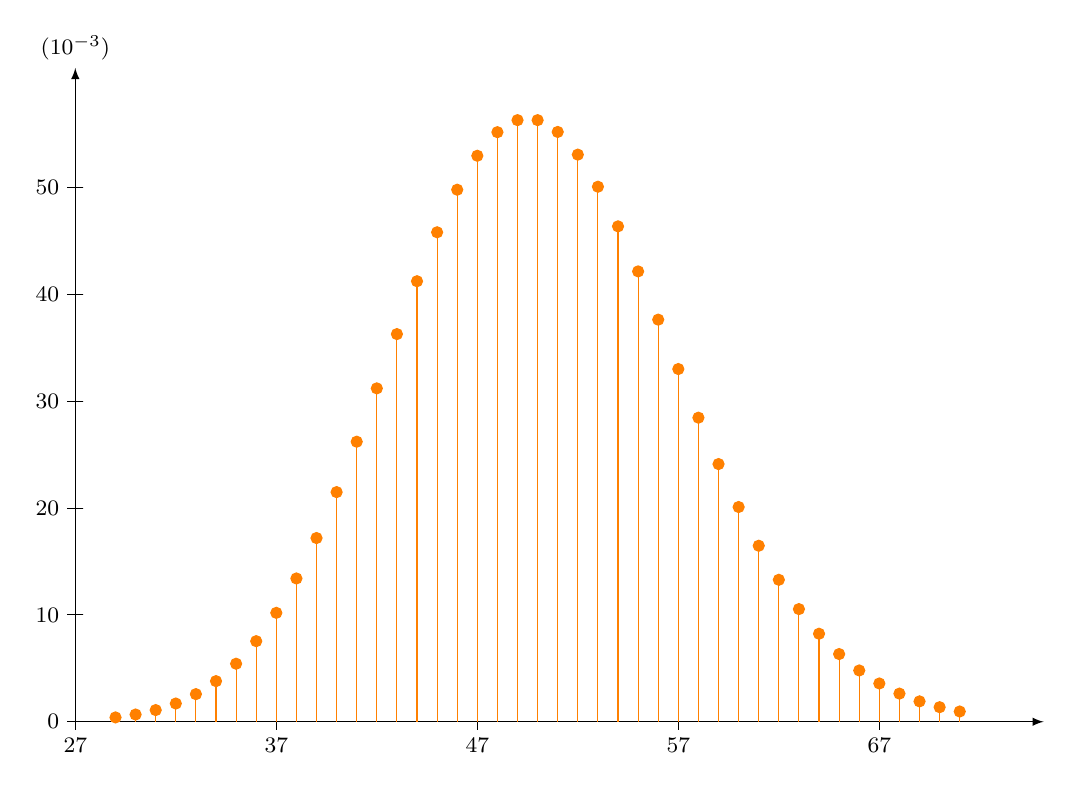
\begin{tikzpicture}[x=0.02553191489361702cm, y=0.013559322033898305cm]
\footnotesize
\draw [-latex] ([xshift=-0mm] 0.0,0) -- ([xshift=3mm] 470.0,0) node[right] {};
\draw (0.0,0) -- +(0mm,1mm) -- +(0mm,-1mm) node[below] {27};
\draw (100.0,0) -- +(0mm,1mm) -- +(0mm,-1mm) node[below] {37};
\draw (200.0,0) -- +(0mm,1mm) -- +(0mm,-1mm) node[below] {47};
\draw (300.0,0) -- +(0mm,1mm) -- +(0mm,-1mm) node[below] {57};
\draw (400.0,0) -- +(0mm,1mm) -- +(0mm,-1mm) node[below] {67};
\draw [-latex] ([yshift=-0mm] 0,0.0) -- ([yshift=3mm] 0, 590.0) node[above] { $(10^{-3})$};
\draw (0,0.0) -- +(1mm,0mm) -- +(-1mm,0mm) node[left] {0};
\draw (0,100.0) -- +(1mm,0mm) -- +(-1mm,0mm) node[left] {10};
\draw (0,200.0) -- +(1mm,0mm) -- +(-1mm,0mm) node[left] {20};
\draw (0,300.0) -- +(1mm,0mm) -- +(-1mm,0mm) node[left] {30};
\draw (0,400.0) -- +(1mm,0mm) -- +(-1mm,0mm) node[left] {40};
\draw (0,500.0) -- +(1mm,0mm) -- +(-1mm,0mm) node[left] {50};
\draw [ycomb, color=orange, mark=*, style=solid] plot coordinates {%
(20.00,4.0632) %   (29.000000,  0.000406)
(30.00,6.7720) %   (30.000000,  0.000677)
(40.00,10.9226) %   (31.000000,  0.001092)
(50.00,17.0665) %   (32.000000,  0.001707)
(60.00,25.8583) %   (33.000000,  0.002586)
(70.00,38.0269) %   (34.000000,  0.003803)
(80.00,54.3242) %   (35.000000,  0.005432)
(90.00,75.4503) %   (36.000000,  0.007545)
(100.00,101.9599) %   (37.000000,  0.010196)
(110.00,134.1577) %   (38.000000,  0.013416)
(120.00,171.9970) %   (39.000000,  0.017200)
(130.00,214.9963) %   (40.000000,  0.021500)
(140.00,262.1906) %   (41.000000,  0.026219)
(150.00,312.1317) %   (42.000000,  0.031213)
(160.00,362.9438) %   (43.000000,  0.036294)
(170.00,412.4362) %   (44.000000,  0.041244)
(180.00,458.2624) %   (45.000000,  0.045826)
(190.00,498.1113) %   (46.000000,  0.049811)
(200.00,529.9057) %   (47.000000,  0.052991)
(210.00,551.9851) %   (48.000000,  0.055199)
(220.00,563.2501) %   (49.000000,  0.056325)
(230.00,563.2501) %   (50.000000,  0.056325)
(240.00,552.2059) %   (51.000000,  0.055221)
(250.00,530.9673) %   (52.000000,  0.053097)
(260.00,500.9125) %   (53.000000,  0.050091)
(270.00,463.8079) %   (54.000000,  0.046381)
(280.00,421.6435) %   (55.000000,  0.042164)
(290.00,376.4674) %   (56.000000,  0.037647)
(300.00,330.2346) %   (57.000000,  0.033023)
(310.00,284.6850) %   (58.000000,  0.028468)
(320.00,241.2585) %   (59.000000,  0.024126)
(330.00,201.0487) %   (60.000000,  0.020105)
(340.00,164.7940) %   (61.000000,  0.016479)
(350.00,132.8984) %   (62.000000,  0.013290)
(360.00,105.4749) %   (63.000000,  0.010547)
(370.00,82.4023) %   (64.000000,  0.008240)
(380.00,63.3864) %   (65.000000,  0.006339)
(390.00,48.0200) %   (66.000000,  0.004802)
(400.00,35.8358) %   (67.000000,  0.003584)
(410.00,26.3499) %   (68.000000,  0.002635)
(420.00,19.0941) %   (69.000000,  0.001909)
(430.00,13.6386) %   (70.000000,  0.001364)
(440.00,9.6047)} %   (71.000000,  0.000960)
 node[right] { };
\end{tikzpicture}
\end{center}
